\problemname{Hesthoppning}
De snela hestarna Hsara och Pascal bor tillsammans i en tvådimensionell hage av
storlek $N$ rader och $M$ kolumner. Hagen är omgiven av ett stort stängsel, men
innanför det så finns det rutor där hestarna kan hoppa fritt. De vill dock båda
undvika att hoppa på rutor där det ligger stora stenar.

För de som spelat schack så är det välkänt att ett hopp går till genom att ta
två steg i en riktning och ett steg i en riktning vinkelrät mot den första. Det
är möjligt att hoppa över stenar, men rutan som man landar i måste vara fri.
Givet hur hagen ser ut, och var hestarna befinner sig från början, så vill de
veta om det är möjligt för dem att träffas. De kan träffas om det finns något
sätt de kan hoppa på så att de hamnar på samma ruta. Hjälp dem att ta reda på
det.

\section*{Input}
Den första raden innehåller heltalen $N$ och $M$, separerade med ett blanksteg.

De nästa $N$ raderna består av $M$ tecken som var och en beskriver hur en ruta
i hagen ser ut. Ett '.' innebär att rutan är tom, '\#' beskriver en ruta med en
sten i, och 'H' betyder att en av hestarna står i den här rutan.

Hagen är omgiven av stängsel. Det är garanterat att indata alltid innehåller
exakt två 'H'-celler.

\section*{Output}
Ditt program ska skriva ut ett ord på en rad - "JA" om hestarna kan mötas på
någon cell och "NEJ" annars.

\section*{Förklaring av exempel}
\begin{figure}[ht!]
\centering
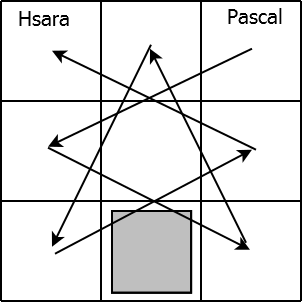
\includegraphics[width=0.25\textwidth]{hestar.png}
\caption{En illustration av Sample Input 2 som visar hur Pascal kan hoppa för att nå Hsara.}
\label{overflow}
\end{figure}

\section*{Poängsättning}
Din lösning kommer att testas på en mängd testfallsgrupper. För att få poäng
för en grupp så måste du klara alla testfall i gruppen.

\begin{tabular}{| l | l | l | l |}
\hline
Grupp & Poängvärde & Gränser \\ \hline
1 & 40 & $3 \le N,M \le 100$ \\ \hline
2 & 60 & $3 \le N,M \le 500$ \\ \hline
\end{tabular}
